\chapter{Kiến thức nền tảng}
\label{Chapter2}
\graphicspath{{Chapter2/Chapter2Figs}}

\textit{Tong chương này, đầu tiên chúng tôi sẽ trình bày về mô hình 
``Auto-Encoders'', một mạng nơ-ron được dùng để học đặc trưng ẩn dựa trên
phương pháp học không giám sát.
Sau đó, chúng tôi giới thiệu và trình bày về nền tảng xác suất 
của ``Variational Auto-encoders'' (VAEs) và lợi ích mang lại của 
mô hình này so với ``Auto-Encoder'' trong tác vụ học đặc trưng ẩn; 
Những điểm lợi này chính là lý do mà chúng tôi tập trung nghiên cứu VAEs. 
Bên cạnh đó, chúng tôi sẽ trình bày về ``Maximum Likelihood Estimation'', 
một phương pháp dùng để đánh giá các tham số của mô hình, đại diện cho các tham số 
của các phân phối xác suất dựa trên dữ liệu huấn luyện. 
Chương này đặc biệt là phần về ``Variational Auto-Encoders'' 
cung cấp những kiến thức nền tảng để có thể hiểu rõ về những đề xuất 
của chúng tôi ở chương kế tiếp.}


% \textit{Bên cạnh đó, chúng tôi sẽ trình bày về ``Log-likelihood fuctions'' - 
% là phép đo mức độ học của mô hình dựa trên các dữ liệu ta quan sát được 
% cũng như các lựa chọn Log-likelihood fucntion cho các bài toán học máy hiện nay.}
% 7->10; 15->20; 15->20; 10->15; 2 (~60)
\newpage

\section{Mô hình rút trích đặc trưng ``Auto-Encoder''}
\label{chap2/sec1}
Mô hình ``Auto-Encoder'' là một mạng nơ-ron truyền thẳng được huấn luyện
để cố gắng sao chép đầu vào của nó thành đầu ra. Bên trong ``Auto-Encoder''
có một lớp ẩn \textbf{\textit{h}} mô tả đặc trưng ẩn, gọi là véc-tơ biểu diễn ẩn đại diện cho đầu vào của nó.

Kiến trúc của một ``Auto-Encoder'' (được minh họa trong hình~\ref{fig_AE}) bao gồm hai phần:
\begin{itemize}
    \item Bộ mã hóa (encoder) ánh xạ véc-tơ đầu vào sang véc-tơ biểu diễn ẩn: 
    \begin{center}
        \begin{math}
            \centering
            \textbf{\textit{h}} = f(x)
        \end{math} 
            
    \end{center}
    \item Bộ giải mã (decoder) có nhiệm vụ cố gắng tái tạo lại véc-tơ đầu vào từ véc-tơ biểu diễn ẩn:
    \begin{center}
        \begin{math}
            \hat{x} = g(\textbf{\textit{h}}) = g(f(x))
        \end{math}
    \end{center}
\end{itemize}

\begin{figure}
    \centering
	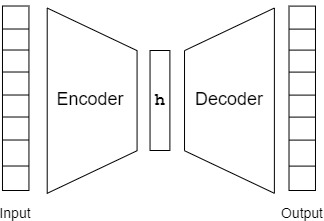
\includegraphics[width=0.6\textwidth]{AE.jpg}
    \caption{Minh họa ``Auto-Encoder''}
    \label{fig_AE}
\end{figure}

``Auto-Encoder'' được huấn luyện bằng cách cực tiểu hóa hàm lỗi là độ sai lệch giữa dữ liệu được tái tạo
với dữ liệu đầu vào. 
\begin{equation}
\label{AE_loss}
    L(x, g(f(x)))
\end{equation}
Các hàm để tính độ lỗi thường được dùng là ``Mean-square error'' hoặc ``Binary cross-entropy''.
Tương tự như các mạng nơ-ron khác, ``Auto-Encoder'' có thể được huấn luyện bằng phương pháp ``Gradient-descent''
với thuật toán lan truyền ngược (``back-propagation'').



Khi thiết kế mô hình, kiến trúc của encoder, decoder
và kích thước của véc-tơ \textbf{\textit{h}} được xem như những siêu tham số của mô hình.
Bằng các cách thiết lập khác nhau, mô hình sẽ có những tính chất khác nhau. 
``Auto-Encoder'' với encoder và decoder là những hàm phi tuyến (cụ thể là mạng nơ-ron với hàm kích hoạt phi tuyến)
với khả năng tính toán quá mạnh hay trường hợp kích thước của véc-tơ \textbf{\textit{h}}
lớn hơn hoặc bằng so với véc-tơ đầu vào sẽ dẫn đến mô hình chỉ học cách sao chép thay vì trích xuất các đặc trưng ẩn từ dữ liệu. 

Thông thường, một ``Auto-Encoder'' sao chép một cách ``hoàn hảo'' đầu vào thành đầu ra
sẽ không có nhiều ý nghĩa. Thay vào đó, ``Auto-Encoder'' được thiết kế với các ràng buộc để không thể
học cách sao chép ``hoàn hảo'' mà chỉ có thể sao chép gần đúng, từ đó ta hy vọng quá trình 
huấn luyện ``Auto-Encoder'' sẽ thu được véc-tơ biểu diễn ẩn có những thông tin hữu ích.

Từ véc-tơ biểu diễn ẩn thu được trong quá trình huấn luyện ``Auto-Encoder'', ta có thể áp dụng mô hình này
như một mô hình trích xuất đặc trưng ẩn từ dữ liệu, làm đầu vào cho các tác vụ khác. 
Hoặc véc-tơ biểu diễn ẩn này có thể áp dụng được trong các tác vụ giảm chiều dữ liệu hỗ trợ cho các tác vụ
lưu trữ, truy vấn, tìm kiếm.

    \subsection{``Undercomplete Auto-Encoder''}
    \label{chap2/subsec11}
    Như đã trình bày trước đó, việc sao chép đầu vào thành đầu ra của ``Auto-Encoder'' không mang nhiều ý nghĩa.
    Ta cần các ràng buộc để có được \textbf{\textit{h}}
    nhận các thuộc tính hữu ích với các ràng buộc khi thiết kế mô hình.
    
    Một cách ràng buộc để mô hình có thể học được các đặc trưng ẩn từ dữ liệu
    là giới hạn véc-tơ đặc trưng ẩn \textbf{\textit{h}} có kích thước nhỏ hơn đáng kể so với véc-tơ đầu vào;
    tính chất này được gọi là ``under-complete''.
    
    Mô hình ``Auto-Encoder'' với kích thước \textbf{\textit{h}} nhỏ hơn đáng kể so với kích thước của véc-tơ đầu vào
    được gọi là ``Undercomplete Auto-Encoder''. Việc giới hạn này sẽ buộc mô hình phải nắm bắt các đặc trưng
    nổi bật nhất.

    Quá trình huấn luyện ``Undercomplete Auto-Encoder'' cũng giống với mô hình ``Auto-Encoder'',
    ta cần cực tiểu hóa hàm lỗi (công~thức~\ref{AE_loss}) là độ sai lệch giữa dữ liệu được tái tạo
    với dữ liệu đầu vào.

    ``Undercomplete Auto-Encoder'' là mô hình tốt để sử dụng cho các tác vụ tiêu biểu của ``Auto-Encoder'' truyền thống
    như trích xuất đặc trưng, giảm chiều dữ liệu 
    bởi vì tính chất ``under-complete'' của mô hình giúp dễ dàng thu được véc-tơ biểu diễn ẩn mang những thông tin hữu ích.


    \subsection{``Denoising Auto-Encoder''}
    \label{chap2/subsec12}
    
    Hàm lỗi của một ``Auto-Encoder'' thông thường sẽ ``phạt'' một mức nhất định với các mẫu dữ liệu được tái tạo lại
    khác với dữ liệu đầu vào. Điều này vô hình chung khuyến khích 
    nghĩa là 
    \begin{math}
        f \circ g
    \end{math}
    là một hàm đồng nhất nếu khả năng tính toán của 
    \begin{math}
        f
    \end{math} 
    và
    \begin{math}
        g
    \end{math}
    cho phép. Nói đơn giản hơn, điều này là việc mô hình sao chép ``hoàn hảo'' đầu vào thành đầu ra của nó.
    Khi đó, véc-tơ biểu diễn ẩn sẽ không có các thông tin hữu ích. 

    Bằng cách thay đổi cách tính toán độ lỗi khi tái tạo lại, cụ thể là thêm nhiễu vào véc-tơ đầu vào, 
    sau đó tính toán độ lỗi là đầu ra được mô hình tái tạo lại so với đầu vào ban đầu như sau:
    \begin{equation}
        L(x, g(f(\tilde{x})))
    \end{equation}
    với 
    \begin{math} \tilde{x} \end{math}
    là véc-tơ đầu vào 
    \begin{math}
        x
    \end{math} 
    được thêm một độ nhiễu, ta có được mô hình ``Denoising Auto-Encoder'' (hình~\ref{fig_DAE}). 
    \begin{figure}
        \centering
        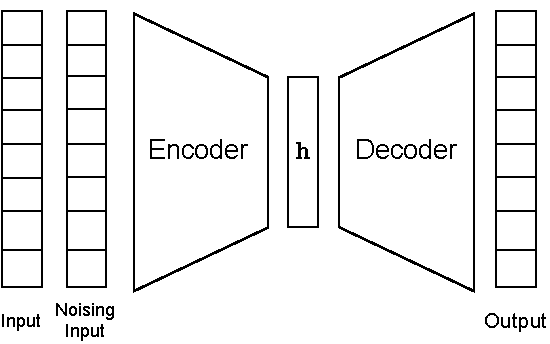
\includegraphics{DAE.pdf}
        \caption{Minh họa ``Denoising Auto-Encoder''}
        \label{fig_DAE}
    \end{figure}
    
    ``Denoising Auto-Encoder'' phải học cách khử độ nhiễu đã được thêm vào véc-tơ đầu vào,
    giảm khả năng sao chép của mô hình.






\section{``Variational Auto-Encoder''} \label{chap2/sec2}
        Variational Auto-encoders (VAEs) là một biến thể đặc biệt của Auto-encoder cơ bản. VAEs, ngoài là một mô hình rút trích đặc trưng ẩn dựa trên phương pháp học không giám sát, còn là một mô hình phát sinh dữ liệu hiệu quả. Khả năng phát sinh thêm dữ liệu là việc dựa trên những đặc trưng ẩn đã học được, VAEs dựa vào những đặc trưng này để thực hiện tác vụ phát sinh dữ liệu. Đây là một điểm khác biệt so với mô hình Auto-Encoder khi mà đặc trưng ẩn học từ Auto-encoder cơ bản không thể được sử dụng để phát sinh. Điều tạo nên sự khác biệt này là bởi đặc trưng ẩn có được từ VAEs là một phân phối xác suất. Auto-encodêr hay kể cả denosing auto-encoder, việc nhận dữ liệu đầu vào, và trích xuất đặc trưng ẩn đều có thể được xem như là một phép chiếu dữ liệu ở chiều không gian cao lên một chiều không gian thấp hơn (thông thường thì số chiều của đặc trưng ẩn dược trích xuất sẽ nhỏ hơn so với dữ liệu đầu vào). Do đó, đặc trưng ẩn này, ta có thể xem như là một điểm dữ liệu mới thể hiện cho dữ liệu ban đầu ở một chiều không gian khác với số chiều thấp hơn. Còn VAEs, thì đặc trưng ẩn không còn là một điểm dữ liệu, thay vào đó sẽ là một ``phân phối xác suất''. Phân phối xác suất là quy luật cho ta biết với mỗi giá trị cụ thể của một đại lượng, một biến số nào đó, sẽ tương ứng với giá trị xác suất là bao nhiêu. 

        Tuy nhiên, bản chất của mô hình Variational auto-encoder được xuất phát từ lĩnh vực xác suất thống kê chứ không phải lĩnh vực khoa học máy tính. Bản chất của một mô hình VAEs là một mô hình đồ thị (graphical models) - là một mô hình dùng để giải thích các mối quan hệ giữa các biến ngẫu nhiên trong xác suất thống kê. Và nền tảng của mô hình là Variation Inference - là một phương pháp cũng thuộc lĩnh vực xác suất thống kê với mục đích có thể ``giải thích'' được dữ liệu mà ta không quan sát được từ những dữ liệu mà ta đã có. Tận dụng sức mạnh của mạng nơ-ron trong lĩnh vực học máy, các hàm số xác suất được thay thành các mạng nơ-ron. Và thông qua việc huấn luyện mô hình để tìm ra bộ trọng số tốt nhất để giải quyết bài toán được giả định mà mô hình cần giải quyết. 

        Do sự liên hệ chặt chẽ với lĩnh vực xác suất, ở mục này, chúng tôi sẽ trình bày về nền tảng xác suất liên quan với mô hình Variational Auto-Encoder, bao gồm các khái niệm, định lý trong lĩnh vực xác suất thống kê để có thể dễ dàng trình bày nội dung của VAEs ở các mục tiếp theo, cũng như là cách huấn luyện cho mô hình VAEs. 
        

    \subsection{Nền tảng xác suất} \label{chap2/subsec21}
        
        

        Mục tiêu của một mô hình trong lĩnh vực học máy là có thể giải quyết được các vấn đề mà ta không có một ``lời giải'' trực tiếp nhưng ta lại có các dữ liệu được ghi lại về vấn đề mà ta quan tâm đến. Một mô hình học máy hiệu quả sẽ cố gắng ``học'' từ dữ liệu, và từ những ``kiến thức'' đã học được có thể đưa ra các ``quyết định'' để giải quyết được vấn đề đó. Để làm được điều này thì thì ta cần tập các dữ liệu liên quan với vấn đề cần giải quyết, và huấn luyện được mô hình để tìm ra được bộ tham số tốt nhất sao cho mô hình 

        \subsubsection{Định lý Bayes và ứng dụng trong lĩnh vực học máy}
        Trong lĩnh vực ``máy học'' và ``thống kê Bayesian'', chúng ta thường quan tâm đến việc thực hiện các phép suy diễn dữ liệu ẩn ta không quan sát được khi cho trước các dữ liệu ta quan đã quan sát được. Ví dụ như một mô hình phát hiện sản phẩm lỗi, thì ta sẽ quan tâm đến việc khi ta đã có các thông tin về sản phẩm, đây là dữ liệu ta đã quan sát được và từ đó ta suy diễn hay còn được gọi là dự đoán về tình trạng của sản phẩm mà tình trạng này chưa quan sát được. Giả sử rằng, ta có $x$ biến ngẫu nhiên thể hiện cho dữ liệu mà ta đã có, và $y$ là biến ngẫu nhiên của dữ liệu mà ta chưa quan sát được. Theo đó, ta sẽ quan tâm đến việc tìm ra được giá trị $y$ cụ thể khi cho trước giá trị $x$. Về xác suất, hay cụ thể ở đây, theo định lý Bayes, nếu ta có $p(x)$ là thông tin mà ta đã nắm được; và một vài mẫu dữ liệu $p(y|x)$ mà ta đã có trong việc thể hiện mối quan hệ giữa $y$ và $x$, cụ thể là giá trị của $y$ khi ta đã có $x$, thì theo công thức Bayes ta có: $$p(x|y) = \frac{p(y|x)p(x)}{p(y)}$$
        Trong đó, $p(x)$ được gọi là ``prior'', ``prior'' thể hiện ``kiến thức'' chủ quan ban đầu của chúng ta trước khi ta có bất kỳ về thông tin nào về liệu ẩn mà chưa quan sát được.
        Ta có thể chọn ``prior'' nào bất kỳ sao cho phù hợp với chúng ta, nhưng một điều chúng ta cần phải đảm bảo đó là ``prior'' phải là có giá trị khác không trên tất cả các giá trị có thể xuất hiện của $x$, kể cả khi giá trị đó rất hiếm khi xảy ra.
        $p(y|x)$ là ``likelihood'', mô tả mối quan hệ giữa $x$ và $y$ liên quan với nhau như thế nào, và trong trường hợp dữ liệu không liên tục (miền giá trị của $x$ và $y$ không phải là một miền giá trị liên tục), thì nó là xác suất của việc giá trị $y$ cụ thể khi ta đã biết về dữ liệu ẩn $x$. Chú ý rằng ``likelihood'' không phải là một phân phối xác suất của $x$, nó chỉ là phân phối cho $y$. Ta gọi $p(y|x)$ là ``likelihood của $x$ (khi cho trước $y$)'' hoặc là ``xác suất của $y$ khi cho trước $x$'' chứ không được gọi là ``likelihood của $y$''\cite{MacKay2003}.
        ``posterior'' $p(x|y)$ sẽ là giá trị mà ta quan tâm theo này quan điểm của Bayes. Nó thể hiện rằng chúng ta có được thông tin gì về $x$ khi ta có dữ liệu về $y$.
        Theo công thức trên, thì ta còn một giá trị nữa đó là $$p(y) = \int {p(y|x)p(x)\text{d}x = \mathrm{E}_X[p(y|x)]}$$ là ``marginal likelihood'' hay còn được gọi là ``evedience''. Trong công thức trên thì kí hiệu $\mathrm{E}$ thể hiện giá trị kỳ vọng của phân phối xác suất. Theo công thức của bayes thì, ``marginal likelihood'' độc lập với dữ liệu ẩn $x$, do đó ``marginal likelihood'' sẽ đóng vai trò đảm bảo giá trị của ``posterior'' sẽ được chuẩn hoá, có nghĩa là ``posterior'' sẽ có khoảng giá trị từ 0 đến 1. Ngoài tác dụng để chuẩn hoá ra thì ``marginal likelihood'' sẽ đóng vai trò trong việc lựa chọn mô hình ``model selection'' (là việc chọn ra mô hình tốt nhất, giữa các mô hình hoặc giữa các bộ siêu tham số). Tuy nhiên, với việc tính ``marginal likelihood'' là một giá trị tích phân, do đó thông thường việc tính toán giá trị chính xác cho ``marginal likelihood'' sẽ không dễ dàng. 

        \subsubsection{Mô hình xác suất}
        \textbf{\textit{Mô hình xác suất}} là một mô hình được dùng để mô tả một phân 
        phối xác suất bằng cách sử dụng một đồ thị để mô tả các biến 
        ngẫu nhiên tương tác với nhau trong phân phối xác suất. Ở đây 
        chúng tôi sử dụng từ ``đồ thị'' là một định nghĩa về cấu trúc 
        dữ liệu được mô tả trong lĩnh vực lý thuyết đồ thị. Đồ thị 
        bao gồm các đỉnh được kết nối trực tiếp với nhau thông qua 
        các cạnh. Vì cấu trúc của mô hình đươc mô tả bằng đồ thị cho 
        nên những mô hình này còn được gọi với một tên gọi khác là 
        ``Graphical model''.
        Mô hình xác suất thể hiện những khía cạnh mà mang tính chất ``chưa chắc chắn'' (uncertain) của một ``thí nghiệm'' dưới dạng của một phân phối xác suất. Ở đây, xét trong quá trình giải quyết một vấn đề nào đó bất kỳ, một thí nghiệm được thực hiện để kiểm chứng lý thuyết, ... thì cụm từ ``chưa chắc chắn'' mang ý nghĩa là chỉ những điểm dữ liệu mà chúng ta chưa quan sát hay chưa thu thập được, do đó về giá trị cụ thể, khoảng dữ liệu và tính chất của những điểm dữ liệu này chúng ta chưa có thể kiểm chứng được. Mô hình xác suất mang lại cho chúng các công cụ để có thể xây dựng một mô hình học, thuật toán học, cách đưa ra dự đoán từ mô hình đã được huấn luyện và cả việc lựa chọn mô hình. Các công cụ này nhất quán và đồng nhất do nó dựa trên nền tảng 


        Mục tiêu của một mô hình học máy hay mô hình học sâu là có thể giải quyết được các vấn đề mà ta không có một cách trực tiếp để giải quyết, tuy nhiên bên cạnh đó lại có dữ liệu được thu thập về vấn đề đó. Điều đó có nghĩa là ta cần xây dựng các mô hình học có thể ``hiểu'' được hình ảnh, âm thanh tiếng nói hay một đoạn văn bản. Nhưng để xây dựng được các mô hình này ta sẽ phải đối mặt với nhiều khó khăn cần giải quyết. Một trong những khó khăn đó là việc dữ liệu ta thu thập được thường có các cấu trúc phức tạp và dữ liệu ở chiều không gian cao, để có thể xử lý được những dữ liệu như vậy là điều không dễ dàng. 

        Điểm mạnh của một mô hình xác suất đó là khả năng có thể giảm được chi phí cho việc thể hiện một mô hình xác suất và cũng như là chi phí cho việc huấn luyện cũng như suy diễn. Cơ chế hoạt động chính của mô hình xác suất cho phép tát cả các phép tính được thực hiện với thời gian thực thi và bộ nhớ hơn so với các mô hình mô hình hoá dữ liệu. Một lợi ích khác trong việc sử dụng mô hình xác suất khác đó là cho phép chúng ta tách biệt các thể hiện của ``kiến thức'' một cách chi tiết từ quá trình huấn luyện hay quá trình suy diễn. Điều này làm cho các mô hình dễ dàng để cài đặt và ``debug''. Chúng ta có thể thiết kế, phân tích và đánh quá thuật toán huấn luyện và thuật toán suy diễn mà có thể áp dụng rộng rãi ở tất cả các loại đồ thị. Một cách độc lập, chúng ta có thể thiết kế các mô hình mà có thể nắm bắt được mối quan hệ mà chúng ta tin rằng nó quan trọng trong dữ liệu mà chúng ta có. Sau đó chugn ta có thể kết hợp các thuật toán và các cấu trúc khác nhau và có các ``tích Đề-Các'' bất kỳ nào mà phù hợp có thể để áp dụng. Tuy nhiên nó sẽ khó hơn trong việc thiết kế một thuật toán ``end-to-end'' cho tất cả các trường hợp.

        \subsubsection{ ``Maximum Likelihood Estimation''}
    \subsection{Phương pháp ``Variational Inference'' } \label{chap2/subsec22}

        Inference là một lớp bài toán để giải quyết vấn đề tìm hiểu về nhưng thứ mà ta biết được dựa trên những thứ mà ta đã biết. Nói một cách khác thì bài toán này là tiến trình để có thể dưa ra kết luận cho một ước lượng, hay khoảng tin cậy hoặc xấp xỉ một phân phối về một ``biến ẩn'' (lateent variable) thường được gọi kết quả trong mẫu dữ liệu, dựa trên một vài các biến mà ta đã quan sát được thường được gọi là nguyên nhân trong mẫu dữ liệu. 

        Một cách cụ thể thì, ``Bayesian inferene'' là quá trình đưa ra các suy diễn thống kê dựa trên ``định lý Bayes''. Phương pháp Bayesian là một phương pháp trong lĩnh vực xác suất thống kê mà ở đó kiến thức biết được biết trước ``prior knowledge'' được mô hình hoá bởi một phân phối xác suất và được cập nhật mỗi khi có một quan sát mới và những thứ mà ta không chắc chắn hay không quan sát được sẽ được mô hình bởi một phân phôi xác suất khác. Một ví dụ kinh diển là về các tham số của bayesian inference, giả định rằng một mô hình mà dữ liệu x được phát sinh từ một phân phối xác suất mà phân phối xác suất này được xác định bỏi các tham số $\theta$, tuy nhiên giá trị của $\theta$ thì ta chưa biết. Bên cạnh đó, ta giả định rằng, ta có một vài kiến thức được biết từ $\theta$ được gọi là ``prior knowledge'', nó có thể là phân phối xác suất $p(\theta)$. Sau đó, mỗi khi ta có một quan sát x mới, ta có thể cập nhật lại ``prior knowledge'' về tham số $\theta$ thông qua định lý Bayes theo công thức :

        trong đó 

        
        Bayesian Inference là một vấn đề thường được phải giải quyết trong các bài toán trong lĩnh vực xác suất thống kê tuy nhiên trong lĩnh vực học máy, nhiều phương pháp được xây dựng dựa trên việc giải quyết vấn đề Bayesian Inference. Ví dụ: ``Gaussian mixture models'' được dùng để giải quyêt bài toán phân lớp, hay ``Latent Dirichlet Allocation'' để giải quyết bài toán phân loại chủ đề văn vản. Và cả hai mô hình kể trên đều được xây dựng dựa trên việc giải quyết bài toán Bayes Inference.  

        \subsubsection{Computational diffficulties}
        Theo công thứ thì để tính toán ``posterior'' ta cần phải có: ``prior'', ``likelihood'' và ``evedience''. Hai giá trị ở trên tử số ta có thể dễ dàng ác định được trong hầu hết các trường hợp vì đó một phần là giả định của chúng ta về mô hình. Tuy nhiên, ở mẫu số ta cần tính:

        để tính giá trị này với dữ liệu ở chiều không gian thấp có thể không gặp nhiều khó khăn, nhưng khi tính toán ở những chiều không gian cao thì nó có thể trở thành một vấn đề nan giải. Khi dữ liệu có số chiều lớn thì việc tính chính xác giá trị ``posterior'' trong thực tiễn thường sẽ là một việc cực kỳ khó khăn và bất khả thi và ta cần một vài kĩ thuật xấp xỉ thường được dùng để giải quyết việc tính ``posterior''. 

        Chúng ta ca cần chú ý thêm một vài khó khăn khác có thể phải đối mặt khi giải quyết bài toán bayesian inference  như là việc lấy ``tổ hợp'' khi dữ liệu là rời rạc thay vì giá trị liên tục. 

        Bài toán bayesian inference thông thường sẽ xuất hiện trong các phương pháp học máy mà giả định rằng có một Graphical model và khi mà cho trước một vài dữ liệu mà ta có thể quan sát được và mục đích của chúng ta là muốn tái tạo lại dữ liệu ẩn của mô hình. Xét ví dụ trong phương pháp Latent Dircichlet Allocation, một phương pháp để xác định chủ đề của một đoạn văn bản. Ta được cho trước một tập ``từ điển'' với kích thước V từ và có T chủ đề có thể có, mô hình này giải định rằng
        \begin{itemize}
            \item Với mỗi chủ đề, tồn tại một phân phối xác suất ``topic-word''  trên toàn bộ tập từ điển (giả định về prior)
            \item Với mỗi đoạn văn bản, có tồn tại một phân phối xác suất ``document-topic'' trên toàn bộ tập các chủ đề (một giả định prior khác)
            \item Với mỗi từ trong trong văn bản được lấy mẫu từ các phân phối giải định ở trên, cụ thể là đầu tiên chúng ta sẽ lấy mẫu một chủ đè từ phân phối xác suất ``document-topic'' của đoạn văn bản, tiếp theo, từ phân phối xác suất ``topic-word'' ta lấy mẫu một từ từ phân phối xác suất đi kèm với chủ đề được lấy mẫu ở bước trước. 
        \end{itemize}
        Tên của phương pháp này là xuất phát từ giả định Dirichlet pior của mô hình. Mục tiêu của mô hình là có thể suy diễn ``latent topic'' từ từ điển ta quan sát được cũng như là có thể phân rã chủ đề của từng đoạn văn bản. Kể cả khi nếu chúng ta không đi sâu vào chi tiết của mô hình LDA, chúng ta có thể nói một cách đại khái rằng với w là một véc-tơ các từ có trong từ điển và z là véc-tơ liên hệ với những từ đó, chúng ta muốn suy diễn được z dựa trên các quan sát từ w theo công thức bayes đó là:

                $\text{có một công thức ở đây}$
 
        
        \subsubsection{Variational inference}
        Variational inference(VI) là một phương pháp thường hay được sử dụng để giải quyết bài toán bayesian inference. Phương pháp này sử dụng hướng tiếp cận là tìm ra xấp xỉ tốt nhất cho một phân phối xác suất bằng cách tìm ra bộ tham số tốt nhất định nghĩa cho phân phối. 

        Phương pháp VI bao gồm việc tìm ra một xấp sỉ tốt nhất cho một mục tiêu là phân phối xác suất giữa một lớp các phân phối xác suất cho trước. Cụ thể hơn, ý tưởng của VI đó là ta định nghĩa một lớp các phân phối xác suất và tìm ra trên đó bộ tham số sao cho ta có đạt được một phần tử gần nhất với mục tiêu của chúng ta tương ứng với một độ lỗi được định nghĩa cụ thể. 

        Ta xét một phân phối xác suất $\pi$ được định nghĩa từ một ``normalisation factor'' C:        
        $$\pi(.) = C \times g(.) g(.)$$
        Tiếp theo, về cho tiết toán học thì ta nếu ta ký hiệu lớp tham số hoá của các phân phối xác suất như sau
        $$\mathcal{F}_\Omega = {f_\omega; \omega \in \Omega} \Omega  \text{tập các tham số có thể có  }$$
        và chúng ta xét độ lỗi E(q,p) giữa hai phân phối xác suất p và q, việc tìm ra bộ tham số tốt nhất được thể hiện bởi:
        $$\omega^* = \text{arg}_{\omega\in\Omega} \text{min}E(f_\omega,\pi) $$

        Nếu chúng ta có thể thối thiểu hoá được bài toán trên mà không cần có một phân phối $\pi$ được chuẩn hoá một cách chi tiết, ta có thể  sử dụng $f_\omega^*$ như là một xấp xỉ để ước lượng thay vì phải tính toán các biểu thức mà gần như không thể tính được khi ở chiều không gian lớn. 
        
        Do đó phương pháp này có thể dễ dàng được áp dụng và mở rộng cho những trường hợp mà ta cần giải quyết một bài toán với quy mô dữ liệu lớn. 
        

        \subsubsection{Kullback-Leiber Devergence}

    \subsection{Độ sai biệt ``Kullback-Leiber Devergence'' giữa hai phân phối xác suất}  \label{chap2/subsec23}